\documentclass[a4paper, 12pt]{article}

\usepackage{dblfnote}
\usepackage[perpage]{footmisc}
\usepackage{indentfirst}
\usepackage{framed}
\usepackage{tikz}
\usepackage{listings}[language=Python]
\usepackage{float}
%\usepackage{multicol}


% Custom colors
\usepackage{color}

%\setcounter{secnumdepth}{0}

\usepackage[top=3cm, bottom=3cm, left = 2cm, right = 2cm]{geometry} 
\geometry{a4paper} 
\usepackage{url}
\usepackage{graphicx} 
\usepackage{amsmath,amssymb}  
\usepackage[hidelinks]{hyperref}
\usepackage[labelformat=empty]{caption}
\usepackage{xepersian}
\settextfont{XB Yas.ttf}
\usepackage[utf8]{inputenc}

%\usepackage{xepersian}

\DeclareFixedFont{\ttb}{T1}{txtt}{bx}{n}{12} % for bold
\DeclareFixedFont{\ttm}{T1}{txtt}{m}{n}{12}  % for normal

\definecolor{deepblue}{rgb}{0,0,0.5}
\definecolor{deepred}{rgb}{0.6,0,0}
\definecolor{deepgreen}{rgb}{0,0.5,0}

\newcommand\pythonstyle{\lstset{
		language=Python,
		basicstyle=\ttm,
		morekeywords={self},              % Add keywords here
		keywordstyle=\ttb\color{deepblue},
		emph={MyClass,__init__},          % Custom highlighting
		emphstyle=\ttb\color{deepred},    % Custom highlighting style
		stringstyle=\color{deepgreen},
		frame=single,                         % Any extra options here
		showstringspaces=false
}}


% Python environment
\lstnewenvironment{python}[1][]
{
	\pythonstyle
	\lstset{#1}
}
{}

% Python for external files
\newcommand\pythonexternal[2][]{{
		\pythonstyle
		\lstinputlisting[#1]{#2}}}

% Python for inline
\newcommand\pythoninline[1]{{\pythonstyle\lstinline!#1!}}




\begin{document}	
\noindent
\begin{minipage}[c]{5cm}
	\baselineskip=.7cm
	\begin{flushright}
		درس : یادگیری ماشین 
		\\
		دانشجو :
		امیرمحمد خرازی
		\\
		شماره دانشجویی :
		40152521002 
		\\
		استاد درس :  
		\href{mrezghi.ir}{دکتر منصور رزقی آهق}
	\end{flushright}
\end{minipage}
\hfill
\begin{minipage}[c]{3cm}
	\begin{center}
		\href{modares.ac.ir}{
			
\includegraphics[width=2cm]{logo.png}}
	\end{center}	
\end{minipage}
\\[1mm]
\hrule depth .5mm \relax
\begin{flushright}
	تمرین سری اول
	\hfill
	دانشکده علوم ریاضی ، گروه علوم کامپیوتر، گرایش داده‌کاوی
\end{flushright}

\hrule depth .5mm\relax

%\tableofcontents
%\newpage
\section*{تمرین اول }
\subsection*{پیش‌گفتار}
	برای پاسخ این تمرین، با توجه به محدودیت های اینترنتی و عدم دسترسی به تمامی محتوای اینترنت، اغلب جواب ها از سایت ویکیپدیا جمع‌آوری شده‌اند. این موضوع که سایت ویکیپدیا
	\footnote{\lr{Wikipedia}}
	 لزوما اطلاعات کامل و درستی را در دسترس قرار نمی‌دهد را قبول دارم ولی با توجه به شرایط و بررسی اطالاعات بدست آمده، نظر بر این شد که مرجع این پاسخ‌ها را، سایت ویکیپدیا، قرار دهم. 

همچنین در خصوص سوال که از دانشجو درخواست شده بود علاوه بر مفهوم، شباهت‌ها و عدم شباهت‌ها ، اشتراکات و تفاوت‌ها و غیره را با مثال بررسی کند، در هر بخش اگر شباهت خاصی با بخش‌های دیگر مشاهده شود، به آن ذکر شده و اگر توانسته باشم مثالی در این خصوص پیدا کنم، آن نیز در همان بخش ذکر شده است. منظور از این بند این است که بخش جدایی برای این بررسی‌ها در نظر گرفته نشده است و در همان جایی که مفهوم این عبارات شرح داده می‌شود، این موضوعات نیز بررسی می‌گردنند. 
\subsection*{
	علم داده
	\footnote{\lr{Data Science}}
}
ابتدا در سال ۱۹۶۲ آقای جان توکی
\footnote{\lr{John Tukey}}
موضوع آنالیز داده را معرفی کرد که بسیار به علم داده امروزی شبیه بود . در سال ۱۹۸۵ در سمیناری که در پکن برگزار شد، فردی به نام جف وو 
\footnote{\lr{C. F. Jeff Wuu}}
برای اولین بار از واژه علم داده به عنوان جایگزینی برای آمار استفاده کرد. البته پیش از آن در سال ۱۹۷۴، 
آقای پیتر ناور
\footnote{\lr{Peter Naur}}
این واژه را به عنوان نامی جایگزین برای علوم کامپیوتر پیشنهاد داده بود.
 بعدا در سال ۱۹۹۲ شرکت کنندگان در نشست آمار که در دانشگاه مونپلیه 
\footnote{\lr{Montpellier}}
برگزار شد، با تلفیق یافته های آماری، آنالیز داده و محاسبات به ظهور یک رشته جدید که بر روی انواع داده‌های متفاوت تمرکز دارد، موافقت کردند. 
تا بدین جا علم داده را بیشتر به عنوان نامی جایگزین مطرح میکردند اما در سال ۱۹۹۸، هایاشی چیکیو
\footnote{\lr{Hayashi Chikio}} 
بر این موضوع که علم داده یک مفهوم جدید و میان رشته‌ای با سه جنبه : طراحی داده، جمع‌آوری و آنالیز است، تاکیید کرد.
نکته جالب در این تاریخچه این است که همزمان در دهه ۱۹۹۰ ، عناوین محبوبی که بر یافتن الگو در دیتاست‌ها تاکیید داشتند شامل کشف دانش 
\footnote{\lr{Knowledge Discovery}}
و داده‌کاوی
\footnote{\lr{Data Mining}}
بودند.


اما امروزه بیشتر ما علم داده را با کمک ویلیام کلیولند 
\footnote{\lr{William S. Cleveland}}
می‌شناسیم. بعد از مقاله ایشان که در سال ۲۰۰۱ چاپ شد و بر گسترش آمار فراتر از تئوری به حوزه های فنی اشاره داشت، علم داده یبشتر و بیشتر مورد استفاده قرار گرفت. 

البته با گذشت این همه مدت هنوز تعریفی از علم داده که مورد تایید همه زمینه‌ها باشد وجود ندارد و برخی آن‌ را یک کلید واژه
\footnote{\lr{Buzzword}}
 در نظر می‌گیرند. 
 کلید واژه به این معنی که در بازه زمانی خاصی محبوبیت دارند. 
 کلان داده‌ها 
 \footnote{\lr{Big Data}}
 نیز یک اصطلاح بازاری مرتبط است. افرادی که با علم داده کار می‌کنند وظیفه دارند که این کلان داده ها را به اطلاعات قابل استفاده شکسته و نرم‌افزار ها و الگوریتم هایی را طراحی کنند که به شرکت‌ها و موسسات برای انتخاب عمل بهینه کمک می‌کند. 
 
 بطور خلاصه علم داده دانشی میان رشته‌ای است که از روش‌های علمی، فرآیند‌ها، الگوریتم ها و سیستم‌ها برای استخراج دانش و فهم از میان داده‌های نویزی، با ساختار یا بدون ساختار  استفاده می‌کند و این دانش بدست آمده را در طیف وسیعی از کاربرد ها اعمال می‌کند. از نمونه موضوعاتی که با علم داده مرتبط هستند می‌توان به داده‌کاوی، یادگیری ماشین و کلان داده اشاره کرد. 
 
 علم داده مفهومی است که آنالیز داده، انفورماتیک، آمار و متد های آن‌ها را متحد می‌کند برای اینکه پدیده های واقعی داده را بفهمد و آنالیز کند و برای اینکار نیز از تکنیک ها و تئوری های متفاوتی که از حوزه‌های مختلفی چون : آمار، ریاضی، علوم کامپیوتر، علوم اطلاعات و غیره بدست آمده‌اند، استفاده می‌کند. 
 
 لذا علم داده یک دانش میان رشته‌ای است که بر روی استخراج اطلاعات از (معمولا) دیتاست‌های بزرگ و اعمال این دانش بدست آمده برای حل مسائل مختلف، تمرکز دارد. این حوزه شامل آماده کردن داده برای آنالیز، فرموله کردن مسائل علم داده، آنالیز داده، ایجاد راه حل‌های داده-محور و ارائه یافته‌ها برای تصمیم‌گیری می‌باشد. برای همین هم هست که از مهارت‌های مختلفی از علوم کامپیوتر، آمار، ریاضی، نمایش داده و یغره استفاده می‌کند. 
 
 بسیاری از آماری‌ها از جمله نیت سیلور
 \footnote{\lr{Nate Silver}}
 بر این موضوع که علم داده یک حوزه جدید نیست، بلکه اسمی دیگر برای آمار است، تاکیید داشتند. اما به هر حال این موضوع مهم است که علم داده ارتباط زیادی بر آمار دارد .
 
 
 \subsection*{داده‌کاوی
\footnote{\lr{Data Mining}} 
} 
در دهه ۱۹۶۰، آماریان و اقتصادی‌ها از اصطلاحاتی چون ماهیگیری داده 
\footnote{\lr{Data fishing}}
یا لایروبی داده
\footnote{\lr{Data dredging}}
برای اشاره به چیزی که آن‌ها آن‌ را عملکرد بد تجزیه داده بدون فرض پیشین
\footnote{\lr{a-priori}}
می‌دانستند، 
استفاده می‌کردند. 
اصطلاح داده‌کاوی در مقاله‌ای که در سال ۱۹۸۳ ازاقتصاددان مایکل لاول 
\footnote{\lr{Michael Lovell}}
 چاپ شد، استفاده شده. 
 اصطلاح داده‌کاوی در دوره ۱۹۹۰ در جامعه پایگاه داده شروع به ظهور کرد. البته برای یک دوران کوتاهی در دهه ۱۹۸۰، عنوان پایگاه داده کاوی 
 \footnote{\lr{Database Mining}}
 استفاده می‌شد. اسامی دیگری که استفاده می‌شدند مانند باستان‌شناسی داده
 \footnote{\lr{data archaeology}}
 ، 
 برداشت اطلاعات
 \footnote{\lr{information harvesting}}
 ،
 کشف اطلاعات
 \footnote{\lr{information discovery}}
،
استخراج دانش 
\footnote{\lr{knowledge extraction}}
و غیره بودند. 
نکته مهم که در پایگاه داده‌ها وجود دارد و به داده‌کاوی نیز بسیار مربوط است، کشف دانش در پایگاه داده 
\footnote{\lr{Knowledge Discovery in Databases}}
یا کی دی دی 
(\lr{KDD})
است که نخست توسط گریگوری پیاتتسکی-شاپیرو 
\footnote{\lr{Gregory Piatetsky-Shapiro}}
 استفاده شد و بعدا در جوامع دیگری نیز چون هوش مصنوعی و یادگیری ماشین محبوبیت زیادی پیدا کرد. 
امروزه اصطلاحات داده‌کاوی و KDD به جای هم استفاده می‌شوند.

بطور خلاصه، داده‌کاوی فرآیند استخراج و کشف الگوها در دیتاست‌های بزرگ با استفاده از متد‌هایی که در اشتراک یادگیری ماشین، آمار و سیستم‌های پایگاه‌ داده هستند، است. 
داده‌کاوی یک زیر رشته میان رشته‌ای از علوم کامپیوتر و آمار است که هدف نهایی آن استخراج اطلاعات با استفاده از روش‌های هوشمند از دیتاست‌ها و تبدیل این اطلاعات به ساختاری قابل درک که در آینده قابل استفاده باشد، است. لذا در همینجا تفاوت آن با علم داده قابل مشاهده است. داده‌کاوی در حقیقت یکی از گام‌های نحلیل در KDD می‌باشد. جدای گام آنالیز، شامل جنبه‌های پایگاه داده و مدیریت داده، پیش پردازش داده، مدل ،  ماتریس ، پیچیدگی، پس پردازش ساختارهای کشف شده، دیداری سازی و آپدیت کردن برخط می‌باشد.

واژه داده‌کاوی یک واژه غلط 
\footnote{\lr{misnomer}}
است چراکه هدف آن استخراج الگو و دانش از داده‌های زیاد است و استخراج از خود داده منظورمان نیست.  همچنین این واژه نیز یک کلید واژه است مانند علم داده و اغلب به هر شکلی از داده‌های بزرگ مقیاس یا فرآیند‌های اطلاعات (جمع‌آوری، استخراج، انبارداده، آنالیز، آمار) و همچنین کاربرد‌هایی از سیستم‌های کامپیوتری کمک به تصمیم
\footnote{\lr{Computer decision support systems}}
شامل هوش مصنوعی (مثل یادگیری ماشین) و هوش اقتصادی و غیره ، اعمال می‌شود.

کار واقعی داده‌کاوی آنالیز اتوماتیک یا نیمه اتوماتیک یکسری داده‌های زیاد برای کشف الگوهای جالب  مثل آنالیز خوشه، یافتن ناهنجاری‌ها، قوانین انجمنی و غیره است .این الگو‌ها بعدا مورد استفاده قرار می‌گیرند اما مسئله مهم اینجاست که جمع‌آوری داده، آماده سازی داده، تفسیر نتیجه و گزارش بخشی از گام داده‌کاوی نیستند ولی متعلق به KDD می‌باشند. 

تفاوت میان آنالیز داده و دادا‌کاوی در اینجاست که آنالیز داده برای آزمون مدل و فرض روی دیتاست استفاده می‌شود. در مقابل داده‌کاوی از یادگیری ماشین و مدل‌های آماری برای یافتن الگو‌های پنهان در داده‌های زیاد استفاده می‌کند.

استخراج الگوها از داده‌ها بصورت دستی از صده‌های گذشته انجام می‌شده اما امروزه از آنجایی که دیتاست‌ها بزرگتر شده‌اند به جای آنالیز دستی، اینکار بصورت اتوماتیک با کمک کشفیاتی که در علوم کامپیوتر صورت گرفته است به ویژه یادگیری ماشین (شبکه‌های عصبی، آنالیز خوشه، الگوریتم‌های ژنتیک، درخت تصمیم، قوانین تصمیم، SVM و غیره) انجام می‌شود. لذا داده‌کاوی فرآیند استفاده از این متد ها روی داده با هدف پیدا کردن الگو‌های مخفی می‌باشد. در داده‌های بزرگ، داده‌کاوی، پلی میان آمار کاربردی و هوش مصنوعی (که معمولا پایه ریاضی را تشکیل می‌دهند) و مدیریت پایگاه داده ایجاد می‌کند. 

اگرچه در سوال از ما در خصوص KDD، مطلبی نخواسته است، برای روشن‌تر شدن مفهوم داده‌کاوی لازم‌ است مختصری از KDD مطرح شود. بطور خلاصه KDD را با ۵ گام می‌شناسیم :
\begin{enumerate}
	\item
	 انتخاب 
	\item
	پیش پردازش
	\item
	تبدیل
	\item
	داده‌کاوی
	\item
	تفسیر و ارزیابی
\end{enumerate} 
 اگرچه لزوما KDD را یا این ۵ گام نمی‌شناسند، ساده‌ترین شکلی که KDD را تفسیر می‌کنند شامل ۳ مرحله : پیش‌پردازش ، داده‌کاوی و ارزیابی نتیجه است.
 
 پیش پردازش یعنی اینکه داده قبل از اینکه قابل استفاده در الگوریتم‌های داده‌کاوی باشد، باید مرتب و تمیز شود.
 
 داده‌کاوی نیز معمولا یکی از این ۶ کار را انجام می‌دهد:
 \begin{enumerate}
 	\item
 	یافتن ناهنجاری‌ها 
 	\item
 	قوانین انجمنی
 	\item
 	خوشه بندی
 	\item
 	طبقه بندی
 	\item
 	رگرسیون
 	\item
 	خلاصه سازی
 \end{enumerate}
 
 از آنجایی که داده‌کاوی می‌تواند سهوا اشتباه استفاده شود و نتیجه ای را ایجاد کند که خیلی خوب است به نظر برسد ولی قابل استفاده روی داده‌های جدید نباشد (مثل بیش برازش
 \footnote{\lr{overfitting}}
  در یادگیری ماشین)، نیاز به ارزیابی نتیجه داریم. برای اینکار نیز از یک مجموعه آزمون استفاده می‌کنیم. مثلا داده‌کاوی سعی دارد تفاوت میان ایمیل های اسپم و واقعی را تشخیص دهد. ابتدا روی یک مجموعه داده آموزش می‌بیند. پس از اینکه آموزش دید و الگوی آموزش دیده بدست آمد، آن را روی مجموعه آزمون که قبلا آن‌ها را ندیده است، اعمال می‌کنند و سپس دقت آن بررسی می‌شود. 
  
   \subsection*{هوش مصنوعی
   \footnote{\lr{Artificial Intelligence}}
	}
 موجودات مصنوعی با هوش در داستان‌های زیادی استفاده شده‌اند. مطالعه استدلال با  فیلسوفان و ریاضیدانان شروع شد.  مطالعه منطق ریاضی منجر به پیدایش تئوری محاسبات توسط آلن تورینگ 
 \footnote{\lr{Alan Turing}}
 شد. در دهه های ۱۹۵۰ دو دید از نحوه پیدایش هوش ماشین 
 \footnote{\lr{Machine Intelligence}}
 ظاهر شد. دید اول ، هویش مصنوعی نمادین 
 \footnote{\lr{SymbolicAI}}
 ، این بود که از کامپیوترها برای ساخت  
 ظاهری نمادین از دنیا و سیستم‌ها که بتواند در خصوص دنیا استدلال کند،
 استفاده شود. موضوعی که بسیار به این دید نزدیک بود، جستجو ابتکاری 
 \footnote{\lr{heuristic search}}
 بود. دید دوم، رویکرد پیوندی 
 \footnote{\lr{Connectionist approach}}
، تلاش بر ایجاد هوش از طریق یادگیری داشت. مثالی از این دید شامل پرسپترون‌ها است. 

رشته هوش مصنوعی در سال ۱۹۵۶ متولد شد و رشد خوبی داشت تا سال ۱۹۷۴ که با ظهور مشکلات جدید، پژوهش‌ها در این حوزه کم رنگ شد. این دوره به زمستان هوش مصنوعی معروف بود چرا که فاند‌های هوش مصنوعی بسیار دشوار پیدا می‌شد. در اوایل دهه ۱۹۸۰، هوش مصنوعی با موفقیت تجاری سیستم‌های خبره
\footnote{\lr{Expert Systems}}
زندگی دوباره گرفت.  اما دوباره در سال ۱۹۸۷ افت کرد و زمستانی دوباره و طولانی‌تر برای هوش مصنوعی شروع شد. در اواخر دهه ۱۹۹۰ و اوایل صده ۲۱ام، هوش مصنوعی کم کم شهرت از دست رفته خود را   از طریق یافتن راه حل های خاص برای مسائل خاص، بدست آورد.
در دهه‌های اول قرن ۲۱ام یادگیری ماشین این رشته را تقریبا پر کرد و به حل بسیاری از مسائل کمک کرد.
 
 هوش مصنوعی یا AI هوشی است که توسط ماشین‌ها نمایش داده می‌شود و در مقابل هوش طبیعی که توسط حیوانات و انسان نمایش داده می‌شود، قرار دارد. پژوهش هوش مصنوعی به مطالعه عوامل هوشمند 
 \footnote{\lr{Intelligent Agents}}
  تعریف می‌شود و به هر سیستمی که پیرامون خود را درک می‌کند و عملی را انجام می‌دهد که به هدفش نزدیک شود، اشاره می‌کند. 
 
 نکته جالب اینجاست که قبلا هوش مصنوعی را به عنوان ماشین‌هایی که رفتار شناختی و ذهن انسان و را شبیه‌سازی میکنند، مانند یادگیری و حل مسائل، می‌شناختند اما امروزه این تعریف توسط اغلب پژوهشگران هوش مصنوعی رد شده است و امروزه آن را به اصطلاحاتی چون عقلانیت
 \footnote{\lr{rationality}}
 و رفتار عاقلانه تعریف میکنند که نحوه بیان هوش را محدود نمی‌کند.
 
  هر چه ماشین‌ها تواناتر می‌شوند، کارهایی که نیاز به هوش دارند معمولا از هوش مصنوعی حذف می‌شوند؛ به این پدیده اثر هوش مصنوعی می‌گویند. برای مثال نویسه‌خوان نوری
  \footnote{\lr{Optical character recognition}}
   یا OCR مکررا از چیز‌هایی که آن‌ها را هوش مصنوعی می‌دانیم مستثنی می‌شوند زیرا که یک تکنولوژی عادی شده‌اند.  
   
   
   هدف سنتی هوش مصنوعی شامل استدلال، دانش، نمایش، برنامه‌ریزی، یادگیری، پردازش زبان طبیعی ، درک و امکان حرکت و تغییر اشیاء بود. توانایی حل یک مشکل دلخواه از هدف‌های بلند مدت این رشته است. لذا مسئله کلی شبیه‌سازی یا ساخت هوش را به زیر مسائل ذکر شده در بالا شکسته‌اند و در ادامه مختصری از هر کدام آورده خواهد شد:
   \begin{enumerate}
   	\item
   	استدلال - حل مسئله :
   	در ابتدا پژوهشگران الگوریتم‌هایی را پیشنهاد دادند که استدلال انسان را بصورت گام به گام تقلید می‌کرد. در اواخر دهه‌های ۱۹۸۰ و ۱۹۹۰ ، روش‌هایی برای حل مسائلی که در آن‌ها عدم قطعیت وجود داشت و یا اطلاعات کامل وجود نداشت ارائه شد.  با گذشت زمان و بزرگتر شدن مسائل، این روش کارایی خود را از دست داد زیرا انسان نیز به ندرت از استدلال های گام به گام استفاده می‌کند.
   	\item
   	نمایش دانش :
   	نمایش دانش و مهندسی دانش به هوش مصنوعی این امکان را می‌دهد تا به سوالات هوشمندانه پاسخ دهد. نمایشی از آنچه که وجود دارد ، مثلا روابط،، مجموعه اشیاء، مفاهیم، و غیره که عامل (هوش مصنوعی)  آن‌ها را تفسیر می‌کند. 
   	
   	\item
   	برنامه ریزی:
   	یک عامل هوش مصنوعی که بتواند برنامه ریزی کند، شرایط دنیا را نمایش می‌دهد، پیشبینی می‌کند اگر عملی انجام شود چه تغییری صورت می‌گیرد و انتخاب می‌کند که چه عملی را انجام دهد که ارزش آن را بیشینه کند. در حالت کلاسیک، عامل فرض دارد خودش در دنیا تنهاست اما اگر این فرض نباشد و عوامل دیگری روی دنیا تاثیر داشته باشند باید این عدم قطعیت‌ها را نیز دخالت دهد. 
   	
   	\item
   	یادگیری :
   	یکی از اساسی ترین مفهومات هوش مصنوعی از شروع این رشته، یادگیری ماشین است. مطالعه الگوریتم‌های کامپیوتری که با گذشت زمان و با کسب تجربه، بطور خودکار بهبود می‌یابند. انواع یادگیری‌ها مانند یادگیری با ناظر (رگرسیون ، طبقه‌بندی) و بدون ناظر (خوشه‌بندی)، یادگیری تقویتی و غیره . 
   	
   	\item
   	پردازش زبان طبیعی :
   	این شاخه به ماشین‌ها این امکان را می‌دهد تا زبان انسان را بفهمد. یک سیستم قوی در این حوزه می‌تواند یک رابط کاربری باشد که دانش را مستقیم از نوشته‌های انسان بدست می‌آورد. 
   	\item
   	درک : 
   	درک ماشین، یعنی توانایی استفاده از ورودی‌های سنسور‌ها (مثل دوربین، میکروفون و غیره) برای استدلال جنبه‌های دنیا؛ مثلا تشخیص گفتار، تشخیص چهره و غیره .
   	  \item
   	  حرکت و دستکاری :
   	  در یک حرف خلاصه می‌شود . روباتیک .
   	  \item
   	  هوش اجتماعی :
   	  سیستم‌هایی که احساسات انسان را تشخیص، تفسیر ، پردازش و شبیه‌سازی می‌کنند. حوزه مرتبط با این موضوع ارتباط انسان-کامپیوتر
   	  \footnote{\lr{Human-Computer Interaction}}
   	  می‌باشد. 
   	  \item
   	  هوش کلی :
   	  یک ماشین با هوش جامع می‌توان مسائل بیشتری را حل کند و به هوش انسان نزدیک تر است. 
   	  
   \end{enumerate} 
   به طور کلی هوش مصنوعی مانند علم داده است یعنی یک رشته جدا است. البته هوش مصنوعی و علم داده اشتراکاتی دارند و شاید این اشتراکات در آمار و یادگیری ماشین بیشتر دیده شود . همین‌طور داده‌کاوی نیز با هوش مصنوعی و علم داده اشتراکاتی دارد ولی هر دو این‌ها مفاهیم جامع‌تر می‌باشند و محتوای زیادی را در بر می‌گیرند. همان‌طور که در بخش قبل ذکر شد، یادگیری ماشین و پردازش زبان طبیعی بخشی از هوش مصنوعی هستند و هوش مصنوعی جامع‌تر از این‌هاست. 
   
   \subsection*{یادگیری ماشین
	\footnote{\lr{Machine Learning}}   
}
اصطلاح یادگیری ماشین در سال ۱۹۵۹ توسط آرتور ساموئل 
\footnote{\lr{Arthur Samuel}}
ساخته شد ، البته در همین دوران نیز هم معنی کامپیوتر‌های خودآموز  استفاده می‌شد. در اوایل دهه ۱۹۶۰ ماشین یادگیری بصورت آزمایشی و با استفاده از حافظه نواری پانچی
\footnote{\lr{punched tape memory}}
، سایبرترون
\footnote{\lr{Cybertron}}
، توسط شرکتی برای آنالیز سیگنال‌های خورشیدی، الکتروگرام و الگو‌های گفتار با استفاده از یادگیری تقویتی ابتدایی  ساخته شد. 

امروزه یادگیری ماشین دو هدف در نظر دارد. یکی اینکه داده را بر طبق مدل ساخته شده، طبقه بندی کند و دیگری برای اتفاقات آینده بر اساس مدل ساخته شده پیش‌بینی ارائه دهد. 

با تلاش‌های علمی، یادگیری ماشین از تلاش‌های دسترسی به هدف هوش مصنوعی، رشد کرد. اگرچه بعدا با تاکیید بیشتر بر روی  رویکرد منطقی و دانش-محور باعث ایجاد بریدگی میان هوش مصنوعی و یادگیری ماشین شد. در دهه ۱۹۹۰ یادگیری ماشین شروع به شناخته شدن به عنوان یک رشته جدید کرد و هدف خود را از رسیدن به هوش مصنوعی  به  رسیدگی به مسائل قابل حل با ماهیت عملی  تغییر داد و تمرکز خودش را از رویکرد‌های نمادین که از هوش مصنوعی به ارث برده بود به متد‌ها و مدل‌هایی که از آمار، منطق فازی و نظریه احتمال قرض گرفته بود، تغییر داد. 

یادگیری ماشین یک رشته تحقیقاتی در خصوص فهمیدن و ساختن روش‌هایی است که یاد بگیرند. یعنی روش‌هایی که به داده نفوذ کرده تا کارایی یکسری فعالیت‌ها را بهبود دهند. همان طور که ذکر شد، یادگیری ماشین را بخشی از هوش مصنوعی در نظر می‌گیرند. الگوریتم های یادگیری ماشین مدل را بر اساس داده‌های آموزش ساخته تا بعدا پیش‌بینی انجام دهند. از الگوریتم‌های یادگیری ماشین در زمینه‌های زیادی چون دارو، فیلتر ایمیل (اسپم و واقعی)، تشخیص گفتار و بینایی کامپیوتر
\footnote{\lr{Computer Vision}}
، جاهایی که الگوریتم‌های مرسوم امکان انجام آن کار خاص را ندارند یا بسیار سخت‌اند، استفاده می‌شود. 


تفاوت میان هوش مصنوعی و یادگیری ماشین معمولا اشتباه فهمیده می‌شود. یادگیری ماشین یاد می‌گیرد و پیش‌بینی می‌کند براساس مشاهدات منفعل 
\footnote{\lr{passive observations}}
؛ این درحالیست که هوش مصنوعی دلالت بر عاملی دارد که با محیط برای یادگیری و انجام عمل مناسب که شانس بدست آوردن هدفش را بیشینه می‌کند، در حال تعامل است .  

امروزه بسیاری همچنان یادگیری ماشین را زیررشته‌ای از هوش مصنوعی در نظر می‌گیرند درحالیکه دیگران می‌گویند همه یادگیری ماشین در هوش مصنوعی نیست بلکه فقط آن بخش هوش آن زیر مجموعه‌ای از هوش مصنوعی حساب می‌شود. 

یادگیری ماشین و داده‌کاوی نیز معمولا متد‌های یکسانی را استفاده می‌کنند و به طور قال توجهی همپوشانی دارند. اما از آنجایی که یادگیری ماشین بر پیش‌بینی بر اساس ویژگی‌های شناخته شده که از داده‌های آموزش یادگرفته است، تمرکز دارد؛ داده‌کاوی بر کشف ویژگی‌هایی که قبلا شناخته نشده‌اند تمرکز دارد. عملا داده‌کاوی از روش‌های یادگیری ماشین با هدف دیگری استفاده می‌کند. از طرفی یادگیری ماشین هم از روش‌های داده‌کاوی به عنوان یادگیری بدون ناظر یا در بخش پیش پردازش داده برای افزایش دقت یادگیری استفاده می‌کند. در یادگیری ماشین، عملکرد معمولا با توجه به توانایی تولید دوباره دانش شناخته شده ارزیابی می‌شود ولی در داده‌کاوی و KDD هدف اصلی یافتند دانشی است که قبلا ناشناخته است. 

یادگیری ماشین همچنین با بهینه‌سازی ارتباط اساسی دارد. بسیاری از مسائل یادگیری ماشین به صورت کمینه کردن تابع زیان 
\footnote{\lr{Loss Function}}
روی داده‌های آموزش عمل می‌کنند.  
تفاوت میان یادگیری ماشین و بهینه‌سازی در هدف کلی سازی ظاهر می‌شود. یعنی بهینه‌سازی تابع زیان را روی داده‌های آموزش کمینه می‌کند ولی یادگیری ماشین هدفش کمینه کردن این تابع روی داده‌هایی است که تا کنون آن‌ها را ندیده است (داده‌های آزمون). 

یادگیری ماشین و آمار نیز از نظر روش‌ها بسیار به هم نزدیک هستند اما در هدف اصلیشان تفاوت دارند. آمار از نمونه یک استنباط آماری جامعه را بدست می‌آورد درحالیکه یادگیری ماشین الگو‌های پیش‌بینی کلی را پیدا می‌کند. در هر صورت برخی از آماردانان روش‌هایی را از یادگیری ماشین بدست آورده‌اند  که به رشته‌ای به نام یادگیری آماری 
\footnote{\lr{Statistical Learning}}
منجر شد.
   
   هدف اصلی یک یادگیرنده این است که بتواند از تجربه خود تعمیم دهد. یعنی در یادگیری ماشین، این توانایی را داشته باشد که روی نمونه‌ها یا کار‌هایی که تاکنون آن‌ها را ندیده است با توجه به تجربه بدست آورده از داده‌های آموزش، با دقت خوب عمل کند. 
   
   برای بهترین عملکرد در خصوص تعمیم این یادگیرنده‌ها، پیچیدگی فرض با پیچیدگی تابع داده‌ها باید همخوانی داشته باشد. بطور واضح تر باید یک مصالحه وجود داشته باشد. و در غیر اینصورت مسائلی چون کم برازش 
   \footnote{\lr{Underfitting}}
   یا بیش برازش
   رخ می‌دهد. از طرفی نیز باید در زمان چندجمله‌ای قابل حل باشد.
   
   معمولا یادگیری ماشین را به دسته‌های متفاوتی تقسیم می‌کنند از جمله یادگیری با نظر که در آن معلم داریم. یعنی هدف پیدا کردن مدلی است که ورودی را به خروجی وصل می‌کند. در یادگیری بدون ناظر برچسب نداریم . عملا خود یادگیری بدون ناظر هدف ماست (یعنی پیدا کردن الگو پنهان) مثل خوشه‌بندی. یادگیری های نیمه ناظر نیز هستند. یادگیری ها تقویتی دسته دیگری از یادگیری ماشین است که در یک محیط پویا صورت می‌گیرد و فیدبک‌هایی را دریافت می‌کند و سعی دارد جایزه خود را بیشینه کند. 
   
   \subsection*{کلان داده
\footnote{\lr{Big Data}}   
}

   کلان داده به دیتاست‌هایی اشاره دارد که بسیار بزرگ هستند یا برای ابزار‌های سنتی پردازش داده بسیار پیچیده هستند. داده‌ با ردیف‌های بیشتر یعنی قدرت آماری بیشتر درحالیکه داده با پیچیدگی بیشتر (یعنی ستون‌های بیشتر) ممکن است به میزان کشف غلط 
   \footnote{\lr{false discovery rate}}
   بیشتر منجر شود. آنالیز کلان داده‌ها شامل چالش‌هایی چون گرفتن داده، ذخیره سازی داده، آنالیز داده، جستجو، اشتراک، انتقال، دیداری‌سازی، درخواست، بروزرسانی، امنیت اطلاعات و منبع داده می‌شود. 
   
   کلان‌داده‌ها ابتدا با سه مفهوم اصلی ساخته شدند : مقدار، گوناگونی و سرعت. بعدا این مفاهیم گسترش یافتند. 
   
   امروزه از کلان داده برای اشاره به تحلیل‌های پیشگویانه و تحلیل‌های رفتار کاربر یا سایر روش‌های پیشرفته تحلیل‌ داده که مقادیر را از کلان داده‌ها استخراج می‌کنند، استفاده می‌شود. 
   
   عنوان کلان داده از دهه ۱۹۹۰ به بعد ، با کمک جان مشی 
   \footnote{\lr{John Mashey}}
   ،استفاده می‌شد. کلان داده‌ها را معمولا شامل آن دسته از دیتاست‌ها هستند که اندازه آن‌ها فراتر از توانایی ابزار‌های شناخته شده برای گرفتن، مدیریت ، پردازش و غیره است .   فلسفه کلان داده شامل داده‌های بدون ساختار، با ساختار و نیمه ساختار می‌باشد ولی تمرکز اصلی آن روی داده‌های بدون ساختار است. 
   
   کلان داده را می‌توان با مشخصات زیر توصیف کرد ( V ها ) :
   \begin{enumerate}
   	\item 
   	Volume 
   	: 
   	مقدار داده تولید یا ذخیره شده. 
   	\item
   	Variety
   	:
   	گونه و طبیعت داده. طبیعت داده از با ساختار به نیمه ساختار و به بدون ساختار تفاوت دارد. 
   	\item
   	Velocity 
   	:
   سرعتی که داده تولید و پردازش می‌شود تا چالش خاص بر طرف شود. کلان داده‌ها معمولا بطور پیوسته تولید می‌شوند.
   \item
   Veracity :
   صحت و اطمینان داده که به کیفیت و ارزش داده اشاره دارد. یعنی عملا کلان داده‌ها نباید فقط زیاد باشند.
   \item
   Value 
   :
   ارزش بدست آمده از پردازش و آنالیز این دیتاست ‌های بزرگ . 
   \item
   Variability 
   :
   شاخصه تغییر فرمت، ساختار و منبع  کلان داده‌. یعنی عملا کلان داده‌ می‌تواند شامل داده‌های با ساختار و بدون ساختار باشد و از منابع گوناگون بیاید.
   \item
   Exhaustive
   :
   آیا کل سیستم 
   گرفته شده است یا خیر. کلان داده‌ها ممکن است همه داده‌ها را از منابعش در اختیار قرار ندهد.
   \item
   Relational
   :
   اگر داده جمع‌آوری شده شامل فیلد‌های رایج که قابل به هم پیوستن و غیره هستند، است.
   \item
   Extensional
   :
   اگر فیلد جدیدی در هر بخش از داده حمع‌آوری شدهبه راحتی  قابل اضافه شدن یا تغییر است.
   \item
   Scalability
   :
   اگر اندازه سیستم انبار کلان داده بطور سریع قابل گسترش و افزایش است. 
   \end{enumerate}  
   
 کلان داده‌ها در شکل‌های مختلف وجود داشته‌اند و کاربرد‌های مختلفی دارند. از جمله در دولت، سود، سلامت ، آموزش ، رسانه ، بیمه، اینترنت اشیاء، فناوری اطلاعات و غیره کاربرد دارد. 
 
 \subsection*{پردازش زبان طبیعی
\footnote{\lr{Natural Language Processing}} 
}
پردازش زبان طبیعی یا NLP یک زیر رشته‌ای از علوم‌کامپیوتر، زبان شناسی
\footnote{\lr{Linguistics}}
و هوش مصنوعی است که بیشتر به تعاملات میان زبان انسان و کامپیوتر مربوط می‌شود. یعنی چگونه کامپیوتر‌ها را برنامه‌ریزی کنیم تا داده‌های زبان طبیعی را آنالیز و پردازش کند. هدف یک کامپیوتری است که بتواند محتویات یک متن را، به همراه تفاوت‌های ظریف زبانی آن‌ها، بفهمد. این تکنولوژی می‌تواند اطلاعات و مفاهیم را که درون متون وجود دارند را استخراج کند و همچنین آن‌ها را نیز مرتب و گروه‌بندی کند. 

 از نمونه چالش‌های پردازش زبان طبیعی می‌توان به تشخیص گفتار، فهمیدن زبان طبیعی و تولید زبان طبیعی اشاره کرد. 
 
 ریشه پردازش زبان طبیعی به دهه ۱۹۵۰ برمی‌گردد. در سال ۱۹۵۰ ، تورینگ در مقاله ای آزمون تورینگ
 \footnote{\lr{Turing Test}}
 را به عنوان معیار هوش ارائه داد. البته در آن زمان این موضوع به عنوان مسئله‌ای جدا از هوش مصنوعی در نظر گرفه نمی‌شد. 
 
 از تاریخچه پردازش زبان طبیعی می‌توان به پردازش زبان طبیعی نمادین در دهه‌های ۱۹۵۰ تا اوایل دهه ۱۹۹۰ اشاره کرد بدین صورت که با داشتن مجموعه‌ای از قوانین، کامپیوتر فهم از زبان طبیعی را با اعمال این قوانین روی داده‌هایی که مشاهده می‌کند، تقلید می‌کند. از دهه ۱۹۹۰ به بعد ، تا دهه ۲۰۱۰، پردازش زبان طبیعی آماری رشد یافت. تا ۱۹۸۰ بیشتر پردازش‌های زبان طبیعی براساس مجموعه‌های پیچیده قوانینی بود که بصورت دستی نوشته می‌شدند. در اواخر دهه ۱۹۸۰انقلابی در این حوزه رخ داد و این انقلاب با معرفی یادگیری ماشین برای پردازش زبان همراه بود. 
 امروزه آنچه در پردازش زبان طبیعی معروف است، پردازش زبان طبیعی عصبی 
 \footnote{\lr{Neural NLP}}
 می‌باشد. در دهه ۲۰۱۰، شبکه‌های عصبی عمیق به پردازش زبان طبیعی کمک کردند. 
 
 

	 	از نمونه فعالیت‌های پردازش زبان طبیعی می‌توان به تشخیص گفتار، تبدیل متن به گفتار و غیره اشاره کرد. همانطور که ویکیپدیا می‌گوید:
	 	
	 	
	  	\begin{quote}
	  		\textquotedblright
	  		چالش اصلی و عمده در این زمینه درک زبان طبیعی و ماشینی کردن فرایند درک و برداشت مفاهیم بیان‌شده با یک زبان طبیعیِ انسانی است. به تعریف دقیق‌تر، پردازش زبان‌های طبیعی عبارت است از استفاده از رایانه برای پردازش زبان گفتاری و زبان نوشتاری. بدین معنی که رایانه‌ها را قادر سازیم که گفتار یا نوشتار تولید شده در قالب و ساختار یک زبان طبیعی را تحلیل و درک نموده یا آن را تولید نمایند. در این صورت، با استفاده از آن می‌توان به ترجمهٔ زبان‌ها پرداخت، از صفحات وب و بانک‌های اطلاعاتیِ نوشتاری جهت پاسخ دادن به پرسش‌ها استفاده کرد، یا با دستگاه‌ها، مثلاً برای مشورت گرفتن به گفت‌وگو پرداخت. هدف اصلی در پردازش زبان طبیعی، ایجاد تئوری‌هایی محاسباتی از زبان، با استفاده از الگوریتم‌ها و ساختارهای داده‌ای موجود در علوم رایانه است. بدیهی است که در راستای تحقق این هدف، نیاز به دانشی وسیع از زبان است و علاوه بر محققان علوم رایانه، نیاز به دانش زبان شناسان نیز در این حوزه می‌باشد. با پردازش اطلاعات زبانی می‌توان آمار مورد نیاز برای کار با زبان طبیعی را استخراج کرد. کاربردهای پردازش زبان طبیعی به دو دسته کلی قابل تقسیم است: کاربردهای نوشتاری و کاربردهای گفتاری. از کاربردهای نوشتاری آن می‌توان به استخراج اطلاعاتی خاص از یک متن، ترجمه یک متن به زبانی دیگر یا یافتن مستنداتی خاص در یک پایگاه داده نوشتاری (مثلاً یافتن کتاب‌های مرتبط به هم در یک کتابخانه) اشاره کرد. نمونه‌هایی از کاربردهای گفتاری پردازش زبان عبارتند از: سیستم‌های پرسش و پاسخ انسان با رایانه، سرویس‌های اتوماتیک ارتباط با مشتری از طریق تلفن، سیستم‌های آموزش به فراگیران یا سیستم‌های کنترلی توسط صدا. در سالهای اخیر این حوزه تحقیقاتی توجه دانشمندان را به خود جلب کرده‌است و تحقیقات قابل ملاحظه‌ای در این زمینه صورت گرفته‌است.
	  		از مهمترین موانع اساسی این حوزه می‌توان به :
	  		۱ ) نیاز به درک معانی: رایانه برای آن که بتواند برداشت درستی از جمله‌ای داشته باشد و اطلاعات نهفته در آن جمله را درک کند، گاهی لازم است که برداشتی از معنای کلمات موجود در جمله داشته باشد و تنها آشنایی با دستور زبان کافی نباشد. 
	  		۲ ) دقیق نبودن دستور زبان‌ها: دستورِ هیچ زبانی آن‌قدر دقیق نیست که با استفاده از قواعد دستوری همیشه بتوان به نقش هریک از اجزای جمله‌های آن زبان پی برد.
	  		
	  		پردازش زبان‌های طبیعی رهیافت بسیار جذابی برای ارتباط بین انسان و ماشین محسوب می‌شود و در صورت عملی شدنش به‌طور کامل می‌تواند تحولات شگفت‌انگیزی را در پی داشته‌ باشد. سیستم‌های قدیمی محدودی مانند SHRDLU که با واژه‌های محدود و مشخصی سر و کار داشتند، بسیار عالی عمل می‌کردند، به‌طوری‌که پژوهشگران را به شدت نسبت به این حوزه امیدوار کرده‌بودند. اما در تقابل با چالش‌های جدی‌تر زبانی و پیچیدگی‌ها و ابهام‌های زبان‌ها، این امیدها کم‌رنگ شدند. مسئلهٔ پردازش زبان‌های طبیعی معمولاً یک مسئلهٔ 
	  		\lr{AI-Complete}
	  		محسوب می‌شود، چرا که محقق شدن آن به‌طور کامل مستلزم سطح بالایی از درک جهان خارج و حالات انسان برای ماشین است.
	  		\textquotedblleft
	  		
	  	\end{quote}

 
 \subsection*{حفاری متن
\footnote{\lr{Text Mining}} 
}
حفاری متن یا داده‌کاوی متن یا تحلیل متن فرآیندی است که در آن اطلاعات با کیفیت از متن استخراج می‌شود و شامل کشف اطلاعات جدید، قبلا ناشناخته می‌باشد. اطلاعات با کیفیت معمولا با تشکیل الگو‌ها و ترندهایی
\footnote{\lr{Trends}}
  از طریق یادگیری الگو‌‌ آماری بدست می‌آید. بر اساس هوتو و همکاران
  \footnote{\lr{Hotho et al}}
   در سال ۲۰۰۵، می‌توانیم میان سه دیدگاه از حفاری متن، تمایز قائل شویم. این سه دیدگاه شامل استخراج اطلاعات، داده‌کاوی و فرآیند KDD می‌باشد. حفاری متن معمولا شامل ساختار سازی ورودی‌های متنی (معمولا تجزیه کردن)، استنتاج الگو‌ها در داده‌های ساختاری و در نهایت ارزیابی و تفسیر خروجی می‌باشد. کیفیت بالا در حفاری متن به معمولا تلفیقی از علاقه، ازتباط
   \footnote{\lr{relevance}}
   و تازگی 
   \footnote{\lr{novelty}}
   اشاره دارد. از نمونه کار‌های حفاری متن می‌توان به گروه‌بندی متون، خوشه‌بندی متن، استخراج مفهوم، آنالیز و تحلیل عقیده، خلاصه‌سازی متون و مدل‌سازی روابط موجودیت‌ها اشاره کرد.
   
   آنالیز متن شامل بازیابی اطلاعات
   \footnote{\lr{Information Retrieval}}
   و آنالیز واژگان
   \footnote{\lr{Lexical Analysis}}
   می‌باشد تا توزیع فراوانی کلمات، الگو‌ها، اطلاعات و غیره را مطالعه کند. تکنیک های داده‌کاوی شامل آنالیز روابط و انجمن‌ها، دیداری‌سازی و تحلیل پیش‌بینی می‌باشد. هدف نهایی، تبدیل متن به داده‌ای برای آنالیز می‌باشد که توسط مواردی چون NLP و یا الگوریتم‌های دیگر انجام می‌گردنند.
   
   حفاری متن امروزه در موارد زیادی توسط دولت، پژوهشگران و غیره استفاده می‌شود. بنابر ویکیپدیا :
   \begin{quote}
   	\textquotedblright
   	یک کاربرد معمول، جهت اسکن مجموعه‌ای از اسناد نوشته شده در یک زبان طبیعی و مدل کردن مجموعه اسناد برای اهداف کلاس‌بندی پیشگویانه یا پرکردن یک پایگاه داده یا ایندکس جستجو با اطلاعات استخراج شده‌است.
   	
   	اصطلاح آنالیز متن یک مجموعه از تکنیک‌های زبانشناسی، آمار و یادگیری ماشینی را توضیح می‌دهد که محتوای اطلاعات منابع متنی را برای هوشمند سازی کسب و کار، آنالیز اکتشافی داده، تحقیقها یا سرمایه‌گذاری ساختار داده و مدل می‌کند. این اصطلاح تقریباً مترادف متن کاوی است. اصطلاح آنالیز متن بیشتر در کسب‌وکار مورد استفاده قرار می‌گیرد در حالی که متن کاوی حوزه کاربرهای قدیمیتر به ویژه تحقیقها علوم وابسته به زندگی و هوشمند سازی دولت‌ها استفاده می‌شود.
   	
   	اصطلاح آنالیز متن همچنان شرح می‌دهد که کاربرد آنالیز متن برای پاسخ به مشکل‌های کسب و کار، چه وابسته یا مستقل از پرس و جو و آنالیزهای میدانی و داده‌های عددی باشد. واضح است که ۸۰ درصد از اطلاعات وابسته به کسب و کار در شکلی بدون ساختار و متنی است. این تکنیک‌ها و فرایندها دانشی، حقایق ، قواعد کسب و کار و ارتباطات  را کشف و ارائه می‌نمایند که در غیر این صورت در ساختاری متنی، غیرقابل نفوذ برای فرایندهای خودکار باقی مانده بودند.
   	\textquotedblleft
   \end{quote}   
  
 
 \section*{تمرین دوم}
 
 \subsection*{پیش‌گفتار}
 فایل‌های پایتون هر بخش در گوگل کولب نوشته شده و لینک اشتراک آن در ادامه هر بخش قرار گرفته است، علاوه بر آن فایل اصلی آن‌ها نیز ارسال شده‌اند ولی پیشنهاد می‌کنم ابتدا کولب آن‌ها را مشاهده کنید.
 
 \subsection*{بیماران پارکینسون}
 
 اغلب اطلاعاتی که در سوال از ما خواسته شده است، به طور کامل در فایل 
\lr{ \pythoninline{parkinsons.names}}
 آورده شده‌اند و در اینجا بطور خلاصه شرح داده می‌شوند. 
 \begin{itemize}
 	\item 
 	مشخصات دیتاست : چند متغیره
 	\footnote{\lr{Multivariate}}
 	\item
 	تعداد نمونه‌ها :  ۱۹۷ (۱۹۵)
 	\item
 	حوزه : سلامت
 	\item
 	نوع ویژگی‌های : 
 	اعداد حقیقی
 	\item
 	تعداد ویژگی‌ها
 	:
 	23
 	\item
 	زمان اهدا : 
 	\lr{2008-06-26}
 	\item
 	وظیفه : طبقه‌بندی
 	\item
 	مقدار گمشده : 
 	ندارد
 \end{itemize}
 
 این دیتاست توسط مکث لیتل
 \footnote{\lr{Max Little}}
 از دانشگاه آکسفورد
 \footnote{\lr{University of Oxford}}
 با همکاری مرکز ملی صدا و گفتار (در دنور
 \footnote{\lr{Denver}}
 )
 که ضبط سیگنال‌های گفتار را برعهده داشت، ساخته شده است. مطالعه اصلی روی روش‌های استخراج ویژگی
 \footnote{\lr{Feature Extraction}}
 برای اختلالات کلی صدا بود. 
 
 اطلاعات دیتاست : این دیتاست شامل محدوده صدا‌های زیستی اندازه‌گیری شده از ۳۱ انسان ، ۲۳ نفر
 با بیماری پارکینسون 
 \footnote{\lr{Parkinson's Disease}}
 (PD)
 . هر ستون از این جدول شامل یک اندازه‌گیری خاص صدا از این افراد می‌باشد. هدف تبعیض قائل شدن میان افراد سالم و ناسالم است. 
 
 فرمت داده از نوع
 \lr{ASCII CSV}
 است. هر یک از ۱۹۵ ردیف CSV به یکی از صدا‌های ضبط شده باز می‌گردد. برای هر مریض ۶ صدا ضبط شده داریم. اسم افراد نیز در ستون اول به همراه شماره صدا ضبط شده آورده شده است. البته به نظرم در اینجا اشتباه کرده است و اینگونه نیست. 
 
 اطلاعات ویژگی‌ها :
 \begin{itemize}
 	\item 
 	name :
 	اسم و شماره ضبط صدا
 	\item
 	\lr{MDVP:Fo(Hz)}
 	:
 	میانگین فرکانس صوتی
 	\item
 \lr{	MDVP:Fhi(Hz)}
 	:
 	بیشینه فرکانس صوتی
 	\item
 	\lr{MDVP:Flo(Hz)}
 	کمینه فرکانس صوتی
 	\item
 	\lr{MDVP:Jitter(\%)}
 	تا
 	\lr{Jitter:DDP}
 	:
 	چندین اندازه از فرکانس‌های اساسی گوناگون
 	\item
 	\lr{MDVP:Shimmer}
 	تا
 	\lr{Shimmer:DDA}
 	:
 	چندین اندازه از دامنه‌های گوناگون
 	\item
 	\lr{NHR,HNR}
 	:
 	دو اندازه از نرخ نویز به اجزای تونال
 	\footnote{\lr{tonal}}
 	در صدا
 	\item
 	status
 	:
 	وضعیت سلامتی بیمار، آنچه که در طبقه‌بندی استفاده می‌شود. ۱ اگر بیمار  و ۰ اگر سالم باشد.
 	\item
 	\lr{RPDE,D2}
 	:
 	دو اندازه پویا غیرخطی پیچیدگی
 	
 	\item
 	DFA
 	:
 	توان مقیاس فراکتال
 	\footnote{\lr{fractal}}
 	سیگنال
 	\item
 	\lr{spread1,spread2,PPE}
 	:
 	سه اندازه غیر خطی از فرکانس‌های اساسی 
 \end{itemize} 
 
 برای استفاده از این دیتاست ابتدا باید کتابخانه‌های لازم را اضافه کنیم برای اینکار کد زیر را اجرا می‌کنیم :
 \begin{latin}
 	\begin{python}
import pandas as pd
 	\end{python}
 \end{latin}
سپس می‌توانیم داده‌های خود را از سایت مورد نظر (یا دانلود کرده یا مستقیما) وارد کد خود کنیم و از آنجایی که در بخش قبل دانستیم جنس آن از نوع CSV است با کد 
\lr{\pythoninline{read_csv}}
که در 
\lr{\pythoninline{pandas}}
موجود است، آن‌را به یک 
\lr{DataFrame}
تبدیل می‌کنیم.
\begin{latin}
	\begin{python}
path = '../Data/Parkinson/parkinsons.data'

data = pd.read_csv(path)
	\end{python}
\end{latin}  
 
 بعد از آن می‌توانیم به راجتی با دو کد زیر، داده‌های نمونه و هدف را از هم جداکنیم. برای اینکار از 
 \lr{\pythoninline{drop}}
 که از ویژگی‌های 
 \lr{\pythoninline{DataFrame}}
است، استفاده می‌کنیم. با اینکار می‌توانیم ستون 
\lr{status}
را از 
\lr{DataFrame}
خود حذف کرده و آنچه باقی می‌ماند (از جنس 
\lr{DataFrame}
)
همان 
\lr{\pythoninline{x}}
های ماست. از طرفی می‌توانیم با 
\lr{\pythoninline{data['status']}}
ستون 
status
را از دیتافریم اصلی دیافت کنیم، منتها جنس خروجی این کد از نوع سری می‌باشد و برای راحتی آن‌را به طریق زیر به یک دیتافریم تبدیل می‌کنیم.
	\begin{latin}
		\begin{python}
x = data.drop(['status'],axis=1)
y = pd.DataFrame({'status': data['status']})
		\end{python}
	\end{latin}
سپس می‌توانیم با دستوراتی چون 
\begin{latin}
	\begin{python}
data.head()
	\end{python}
\end{latin}

\begin{latin}
	\begin{python}
print("Type : " , type(data) , "\n\nShape" , data.shape  )
	\end{python}
\end{latin}
\begin{latin}
Type :  <class 'pandas.core.frame.DataFrame'> 

Shape (195, 24)
\end{latin}

مشخاصت دیتافریم اولیه و کلی را نمایش دهیم : همانطور که مشاهده می‌شود ۱۹۵ ردیف شامل ۲۴ ستون است که ستون 
status
آن متغیر وابسته و بقیه متغیر‌های مستقل هستند. یعنی 
status
به مقادیر x وابسته است.
البته دستوراتی چون 
\begin{latin}
	\begin{python}
data.info()
data.describe().T
	\end{python}
\end{latin}
نیز اطاعات مفیدی از نوع داده‌ها و تعداد، بیشینه، کمینه، میانگین، انحراف از معیار و غیره هر ستون به ما می‌دهند.

همچنین می‌توان بطور مشابه : 
\begin{latin}
	\begin{python}
x.head()
	\end{python}
\end{latin}

\begin{latin}
	\begin{python}
print("Type : " , type(x) , "\n\nShape" , x.shape)
# x = x.values # to change to numpy array
	\end{python}
\end{latin}
\begin{latin}
Type :  <class 'pandas.core.frame.DataFrame'> 

Shape (195, 23)
\end{latin}


\begin{latin}
	\begin{python}
y.head()		
	\end{python}
\end{latin}

\begin{latin}
	\begin{python}
print("Type : " , type(y) , "\n\nShape" , y.shape)
# y = y.values # to change to numpy array		
	\end{python}
\end{latin}
\begin{latin}
Type :  <class 'pandas.core.frame.DataFrame'> 

Shape (195, 1)
\end{latin}
 
 را برای متغیر‌های x و y نمایش داد. می‌توان آن‌ها را نیز به آرایه تبدیل کرد که در اینجا اینکار انجام نشده است. می‌بینیم که y شامل یک ستون 
 status
 و 
 x 
 شامل سایر ستون‌ها (۲۳) می‌باشد.
 
 پیشنهاد می‌شود کد مربوط به این قسمت را 
 مشاهده و اجرا نمائید.
 
 در خصوص بخش دیگر این سوال که از دانشجو خواسته شده است سه کلاس‌بندی در سه مقاله (بعد از ۲۰۱۸) را با هم فقط بررسی کند، جدول زیر آورده خواهد شد.
 
\begin{center}
\begin{tabular}{|clclc|}
	\hline
	\multicolumn{5}{|c|}{طبقه‌بندی بیماری پارکینسون}                 \\ \hline
	\multicolumn{2}{|c|}{DOI} & \multicolumn{2}{c|}{روش} & 
	بهترین دقت 
	       \\ \hline
	\multicolumn{2}{|c|}{\lr{\href{https://doi.org/10.1109/ACCESS.2019.2936564}{10.1109/ACCESS.2019.2936564}}} 
	 & \multicolumn{2}{c|}{
	یادیگری عمیق و شبکه‌های عصبی پیچشی
	%\footnote{\lr{Convolutional Neural Networks}} 
 	}  
	 & \lr{82.50}         
	 \\ \hline
	 \multicolumn{2}{|c|}{\lr{\href{https://doi.org/10.1109/EBBT.2019.8741725}{10.1109/EBBT.2019.8741725}}} 
	 & \multicolumn{2}{c|}{ماشین‌های یادگیری هیبریدی، تلفیق
	جنگل تصادفی
	%\footnote{\lr{Random Forests classification}}
	و 
	\lr{SMOTE}
		 
 }  
	 & \lr{94.89}        
	 \\ \hline
	 \multicolumn{2}{|c|}{\lr{\href{https://doi.org/10.32604/iasc.2022.022037}{10.32604/iasc.2022.022037}}} 
	 & \multicolumn{2}{c|}{
	 6 روش از جمله جنگل تصادفی و KNN  و درخت تصمیم
 }  
	 & \lr{97.00 }
	 \\ \hline
\end{tabular}
\end{center}
البته لازم است این موضوع را ذکر کنم که در سه مقاله بالا روش‌ها تعمیم یافته شده‌اند و همچنین دقت بدست آمده‌ای که در جدول بالا ذکر شده است، بالاترین دقتی است که بدست آمده و دقت میانگین این طبقه‌بندی‌ها نمی‌باشند.

\subsection*{NetworkX}

از این کتابخانه برای رسم گراف استفاده می‌کنی. ابتدا کتابخانه‌های لازم را اضافه می‌کنیم.
\begin{latin}
	\begin{python}
import numpy as np
import ast
import pandas as pd
import matplotlib.pyplot as plt
import networkx as nx
	\end{python}
\end{latin}

سپس لازم از محتویات فایل‌های 
\lr{\pythoninline{txt}}
را فراخوانی می‌کنیم. ابتدا آن‌ها را با حالت 
\lr{\pythoninline{read-only}}
باز می‌کنیم. سپس خط اول که تنها خط آن‌ است را می‌خوانیم
\lr{\pythoninline{.read()}}
و در نهایت با کمک کتابخانه 
ast
آن‌را به لیست تبدیل می‌کنیم. این کار را برای هر دو فایل انجام می‌دهیم.

\begin{latin}
	\begin{python}
path_edge_idx  = '../Data/NetworkX/edge_idx.txt'
path_node_lbls = '../Data/NetworkX/node_lbls.txt'

edge_idx  = ast.literal_eval(open(path_edge_idx , 'r').read())
node_lbls = ast.literal_eval(open(path_node_lbls, 'r').read())
	\end{python}
\end{latin}
 
 سپس می‌توانیم گراف را بسازیم. برای اینکار بعد از ساخت اولیه محیط گراف، یال‌های آن‌را که در فایل 
 \lr{\pythoninline{edge_idx}}
 موجود است، به آن اضافه می‌کنیم. با اینکار نود های مربوطه نیز اضافه می‌شوند. ولی اگر نودی هیچ یالی نداشته باشد، با این روش اضافه نمی‌شود. از آنجایی که ۳۵ نود (از ۰ تا ۳۴) داریم، این تعداد را نیز به صورت یک لیست به نود‌های گراف اضافه می‌کنیم. البته در اینجا این حرکت لزوم نداشت.
 \begin{latin}
 	\begin{python}
 G = nx.Graph()
 G.add_edges_from(edge_idx)
 G.add_nodes_from(range(0,35)) # not necessary
 	\end{python}
 \end{latin}

سپس می‌توانیم اطلاعات گراف را همانطور که سوال خواسته برای خود نمایش دهیم.
این گراف شامل ۳۵ نود و ۷۴ یال می‌باشد.
\begin{latin}
	\begin{python}
nx.info(G)
	\end{python}
\end{latin}


می‌توانیم این اطلاعات را نیز از نحوه‌های دیگری بدست آوریم:
\begin{latin}
	\begin{python}
print("Graph Edges : ", G.edges)
print("Number of Edges : ", len(G.edges))
print("Graph Nodes : ", G.nodes)
print("Number of Nodes : ", len(G.nodes))
print("Each node's Degree : ", G.degree)
	\end{python}
\end{latin}
با اجرای این کد در محیط پایتون، ابتدا لیستی از تاپل‌های یال‌ها و سپس تعداد یال‌ها نوشته می‌شود. لیستی از نود‌ها و تعداد نودها در ادامه آورده می‌شوند. درجه هر نود هم بصورت یک تاپل که اولین مقدار ان عنوان نود و مقدار دوم آن درجه نود است، آورده می‌شود.

می‌توان برای هر نود یا گره همسایه تعریف کرد بدین معنی که نود مورد نظر با آن نود ارتباط دارد (یال میان آن‌ها برقرار است). بدین صورت می‌توانیم همسایگان هر نود را نمایش دهیم و بررسی کنیم که آیا نودی بدون همسایه است یا خیر . این موضوع با روش‌های دیگری چون
\lr{\pythoninline{G.adj}}
نیز قابل انجام است.
\begin{latin}
	\begin{python}
for node in G.nodes:
	print("Node ", node ,
		 "Neighbors are (have a connection with) : ",
		  end = " ")
	for neighbor in G.neighbors(node):
		print(neighbor, end = " ")
	print("")
	\end{python}
\end{latin}

اما برای اینکه به هدف اصلی سوال برسیم باید بخش‌های زیر را پیاده‌سازی کنیم. اگر بخواهیم برچست هر نود را با استفاده از فایل
\lr{\pythoninline{node_lbls.txt}}
بدست بیاوریم، نیاز به یک دیکشنری داریم. لذا برای هر نود در گراف، مقدار برچسب‌اش را در دیکشنری آن ذخیره می‌کنیم.  از طرفی نوشتن اعداد زیاد روی تصاویر جنبه خوش‌آیندی ندارد و بهتر است از رنگ‌های متفاوت برای برچسب‌های متفاوت استفاده شود. برای اینکار مجموعه رنگی تعریف می‌شود که برای هر نود در گراف اگر برچسب آن ۱ بود سبز رنگ و اگر ۰ بود قرمز می‌شود. 

در سوال از ما خواشته شده است که اندازه هر نود بر اساس درجه آن تغییر کند. برای اینکار لیستی از اندازه‌ها به عنوان 
\lr{\pythoninline{_node_size_1}}
می‌سازیم که در آن هر نود به اندازه‌اش وصل می‌شود. یعنی شماره نود‌ها از ۰ تا ۳۴ است لذا مقدار عنصر ۰ام این لیست برابر با درجه راس ۰ است. از آنجایی که این مقادیر کم هستند، یک عدد دلخواه در همه آن‌ها ضرب می‌شود تا جنبه ظاهری بهتری پیدا کند. این مقدار دلخواه را با 
\lr{\pythoninline{weight}}
نمایش می‌دهیم. از طرفی در آخرین درخواست سوال از ما خواسته شده است تا در محاسبه اندازه نود‌ها، آن همسایگانی را در نظر بگیریم که از یک برچسب یکسان هستند یعنی اگر نود اصلی ما برچسب ۱ دارد، فقط آن تعداد همسایگانی مد نظر است که برچسب آن‌ها ۱ است. برای اینکار برای هر نود اندازه ۰ در نظر گرفته می‌شود، سپس با محاسبه هر همسایه و مقدار برچسب آن، اندازه آن افزایش می‌یابد. در نهایت مانند روش قبل، در یک عدد دلخواه ضرب می‌شود. این روش با عنوان
\lr{\pythoninline{_node_size_2}}
در کد آورده شده است.
\begin{latin}
	\begin{python}
labels_dict = {}
for node in G.nodes:
	labels_dict[node] = node_lbls[node] 

_node_color = []
for node in G.nodes:
	if node_lbls[node]== 1:
		_node_color.append('springgreen')
	else:
		_node_color.append('lightcoral')

_node_size_1 = []
weight = 15
for node in G.degree:
	_node_size_1.append(node[1]*weight)


_node_size_2 = []
weight = 15
for node in G.nodes:
	size = 0
	for neighbor in G.neighbors(node):
		if node_lbls[neighbor] == node_lbls[node]:
		size+=1
	_node_size_2.append(size*weight)
	\end{python}
\end{latin} 

در ادامه لازم است این گراف ها را دیداری‌سازی کنیم. کد اصلی برای تولید یک گراف ساده بدون هیچگونه برچسب یا تغییر رنگ و اندازه. تنها با کمک یال‌ها.
\begin{latin}
	\begin{python}
plt.figure(1)
nx.draw_networkx(
	G,
	node_color='springgreen',
	edge_color='skyblue',
	pos = nx.circular_layout(G),
	with_labels = False
)
plt.show()
	\end{python}
\end{latin}

\begin{figure}[H]
	\begin{center}
		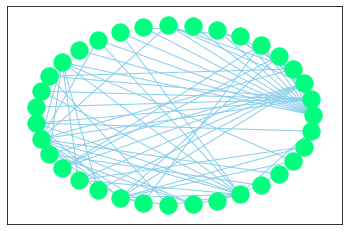
\includegraphics[scale=0.8]{fig1.png}
\end{center}
\caption{گراف ابتدائی}
\end{figure}
می‌توانیم برچسب هر نود را به آن اضافه کنیم و نتیجه آن گراف زیر می‌باشد:
\begin{latin}
	\begin{python}
plt.figure(2)
nx.draw_networkx(
	G,
	node_color='springgreen',
	edge_color='skyblue',
	pos = nx.circular_layout(G),
	labels = labels_dict,
	with_labels = True
)
plt.show()
	\end{python}
\end{latin}
\begin{figure}[H]
	\begin{center}
		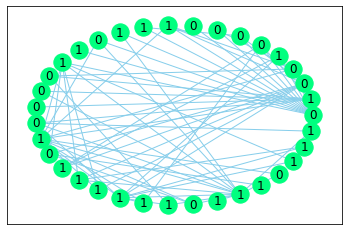
\includegraphics[scale=0.8]{fig2.png}
	\end{center}
\caption{گراف ابتدائی برچسب‌دار}
\end{figure}
می‌توان بجای عدد از رنگ برای تمایز ۰ و ۱ های برچسب‌ها استفاده کرد:
\begin{latin}
	\begin{python}
plt.figure(3)
	nx.draw_networkx(
	G,
	node_color= _node_color,
	edge_color='skyblue',
	pos = nx.circular_layout(G),
	with_labels = True
)
plt.show()
	\end{python}
\end{latin}
\begin{figure}[H]
	\begin{center}
		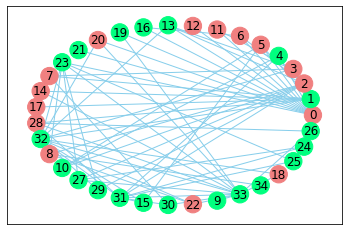
\includegraphics[scale=0.8]{fig3.png}
	\end{center}
\caption{گراف رنگارنگ برچسب‌دار}
\end{figure}
می‌توان اندازه هر نود را با روش اولی، یعنی بر اساس درجه آن ، تغییر داد:
\begin{latin}
	\begin{python}
plt.figure(4)
nx.draw_networkx(
	G,
	node_size = _node_size_1,
	node_color= _node_color,
	edge_color='skyblue',
	pos = nx.circular_layout(G),
	with_labels = False
)
plt.figure(5)
nx.draw_networkx(
	G,
	node_size = _node_size_1,
	node_color= _node_color,
	edge_color='skyblue',
	pos = nx.circular_layout(G),
	with_labels = True
)
plt.show()
	\end{python}
\end{latin}
\begin{figure}[H]
	\begin{center}
		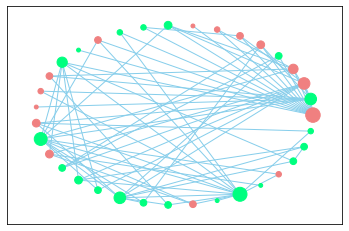
\includegraphics[scale=0.6]{fig4.png}
		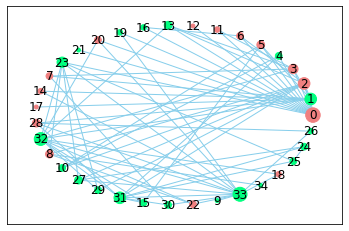
\includegraphics[scale=0.6]{fig5.png}
	\end{center}
	\caption{گراف رنگارنگ با اندازه متفاوت بر اساس درجه}
\end{figure}

می‌توان اندازه را با روش دوم تغییر داد، یعنی بر اساس تعداد همسایگانی که برچسب مشابه دارند. 
\begin{latin}
	\begin{python}
plt.figure(6)
nx.draw_networkx(
	G,
	node_size = _node_size_2,
	node_color= _node_color,
	edge_color='skyblue',
	pos = nx.circular_layout(G),
	with_labels = False
)
plt.figure(7)
nx.draw_networkx(
	G,
	node_size = _node_size_2,
	node_color= _node_color,
	edge_color='skyblue',
	pos = nx.circular_layout(G),
	with_labels = True
)
plt.show() 
	\end{python}
\end{latin}
\begin{figure}[H]
	\begin{center}
		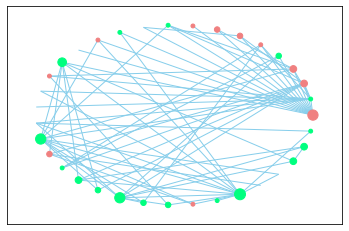
\includegraphics[scale=0.6]{fig6.png}
		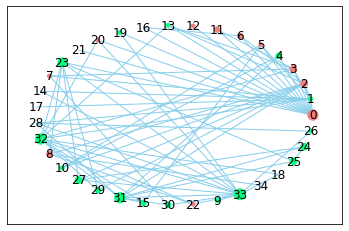
\includegraphics[scale=0.6]{fig7.png}
	\end{center}
	\caption{گراف رنگارنگ با اندازه متفاوت بر اساس برچسب همسایه}
\end{figure}

برای راحتی پیشنهاد می‌کنم کد‌های این بخش را که در پوشه کد هستند، مشاهده و بررسی کنید. 
\subsection*{Pavia}
داده‌هایی که در این بخش استفاده می‌شود مستقیم از خود سایت جمع‌آوری شده‌اند. یعنی از همان لینک
\linebreak 
\href{https://rslab.ut.ac.ir/data}{\lr{Pavia University Scene}}
در بخش 
۳-۲
. و لذا فرمت فایل‌ها 
\lr{\pythoninline{.mat}}
می‌باشد.

فایل اول شامل 
\lr{\pythoninline{PaviaU.mat}}
می‌باشد. تصاویر فراطیفی
\footnote{\lr{HCI}}
 دانشگاه پاویا توسط سنسور‌های ROSIS گرفته شده‌اند. این تصاویر شامل ۱۰۳ باند طیفی، ۶۱۰ در ۳۴۰ پیکسل می‌باشد؛ اما نمونه‌های طیف تصاویر هیچ اطلاعاتی ندارد و لذا ۰ تعریف شده‌اند و قبل از آنالیز دور ریخته می‌شوند. رزولوشن هندسی آن ۱.۳ متر است و حقیقت اصلی این تصاویر فراطیفی به ۹ کلاس خلاصه می‌شود.
  
 این کلاس‌ها شامل آسفالت، درخت ، سایه و غیره می‌باشد.

  فایل دیگر 
  \lr{\pythoninline{PaviaU_gt.mat}}
  می‌باشد. دیداری سازی حقیق اصلی 
  \footnote{\lr{ground truth}}
  این داده‌های فراطیفی است. بعدا در عکس مشخص می‌شود که هرچه رنگ آن روشن تر شود، به یکی از آن ۹ مورد نزدیک تر می‌شود و نقاط کاملا تیره، هیچ اطلاعاتی موجود نیست.
  
  تصویربرداری فراطیفی نوعی از تصویربرداری طیفی است که مانند سایر انواع تصویربرداری طیفی داده‌ها را از بخشی یا تمام طیف الکترومغناطیسی گردآوری و پردازش می‌کند. در حقیقت یک شیء در طول موج‌ها ی مربوط به رنج فراطیفی که بالاتر از طول موج‌های طیف مرئی هستند مورد تصویر برداری قرار می‌گیرد . هدف اصلی در تصویر برداری فرا طیفی، بدست آوردن محتوای طیفی یا به اصطلاح اثر طیفی برای هر پیکسل از تصویر است . 



برخلاف چشم انسان که تنها می‌تواند نور قابل دیدار در سه باند (قرمز، سبز و آبی) را ببیند، تصویربرداری فراطیفی دامنهٔ دید را به باندهای بسیار بیشتری گسترش می‌دهد .این نکته حائز اهمیت است که رنگ‌هایی که چشم انسان می بیند در واقع بازتاب طول موج‌های متفاوت در رنج طیف مرئی انسان است و وقتی که در مورد گسترش قدرت دید فرای این طیف مرئی صحبت می کنیم این تفاوت و برتری خود را به شکل اعداد به ما نشان می دهند و نه رنگ‌ها ! چون بالاخره چشم انسان رنج مرثی را می بیند . تفاوت ظاهری در این است که ثصاویر فراطیفی گرفته شده با به اصطلاح رنگ ساختگی آشکارسازی می‌شوند .

 \begin{latin}
	\begin{center}
		\begin{tabular}{|c|c|c|}
			\hline
			label & class & Samples 
			\\\hline
			1 & Water & 824
			\\\hline
			2  & Trees & 820
			\\\hline
			3 & Asphalt & 816
			\\\hline
			4 & Self-Blocking Bricks & 808
			\\\hline
			5 & Bitumen & 808
			\\\hline
			6 & Tiles & 1260 
			\\\hline
			7 & Shadows & 476
			\\\hline
			8 & Meadows & 824
			\\\hline
			9 & Bare Soil & 820
			\\\hline
		\end{tabular}
	\end{center}
\end{latin}

تصاویر فراطیفی کاربرد‌های زیادی دارند اگرچه ابتدا برای زمین‌شناسی و داده‌کاوی ساخته شده بودند.  از نمونه کاربرد‌های آن می‌توان به کشاورزی، تجزیه و مرتب‌سازی زباله، مراقبت از چشم، پردازش غذا،  کانی‌شناسی
\footnote{\lr{Mineralogy}}
، نظارت، فضانوردی، تصویربرداری شیمیایی، محیط زیست و مهندسی عمران اشاره کرد. لذا کاربرد‌های زیادی در رشته‌های مختلفی دارند. 



اما برای خواند این فایل‌ها در پایتون ابتدا کتابخانه‌های لازم را اضافه می‌کنیم :
\begin{latin}
	\begin{python}
from scipy.io import loadmat
import numpy as np
import pandas as pd
import random
import matplotlib.pyplot as plt
	\end{python}
\end{latin}
سپس مسیر‌های این داده‌ها را مشخص و آن‌ها را می‌خوانیم:
\begin{latin}
	\begin{python}
path_pavia   = '../Data/Pavia/PaviaU.mat'
path_paviagt = '../Data/Pavia/PaviaU_gt.mat'
path_npy     = '../Data/PVI/pavia.npy'


pavia       = loadmat(path_pavia)
paviagt     = loadmat(path_paviagt)
pavia_npy   = np.load(path_temp)
	\end{python}
\end{latin}
می‌توانیم بعدا با کد‌هایی چون
\lr{\pythoninline{pavia}}
و
\lr{\pythoninline{paviagt}}
یا
\lr{\pythoninline{pavia_pnpy}}
فایل‌های خوانده شده را بررسی کنیم. اما در این فایل‌ها (دو فایل اول) تنها به بخش خاصی از آن نیاز داریم. لذا این بخش‌ها را از آن جدا می‌کنیم. سپس می‌توانیم ابعاد داده بدست آمده را چاپ کنیم و آن‌را بررسی کنیم.
\begin{latin}
	\begin{python}
pavia = pavia['paviaU']
pavia.shape
	\end{python}
(610, 340, 103)
\end{latin}
\begin{latin}
	\begin{python}
paviagt = paviagt['paviaU_gt']
paviagt.shape
	\end{python}
(610, 340)
\end{latin}
\begin{latin}
	\begin{python}
pavia_npy.shape
	\end{python}
(1096, 715, 102)
\end{latin}

فایل gt شامل باند‌های یکتایی است که این تقاط دارند. با کمک آن می‌توانیم تصویری مشترکی از باند‌ها در هر نقطه بصورت زیر رسم کنیم:
\begin{latin}
	\begin{python}
plt.figure(1)
plt.imshow(paviagt, cmap='inferno')
plt.colorbar()
plt.axis('off')
plt.title('Ground Truth')
plt.gca().legend(np.unique(paviagt),
	loc='upper left')
plt.show()
	\end{python}
\end{latin}
\begin{center}
		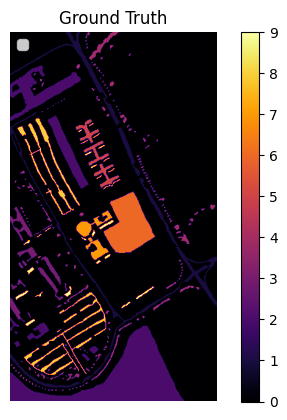
\includegraphics[scale=0.7]{fig8.png}
\end{center}
می‌توانیم در اینجا آن‌ها را به مقیار مورد نظر ببریم که من اینکار را نکردم. می‌توانیم تصویر هر بخش را نیز بصورت زیر بدست آوریم. 
\begin{latin}
	\begin{python}
pavia[:,:,0]
	\end{python}
\end{latin}
سپس می‌توانیم این تصویر بدست آمده را چاپ کنیم.

	\begin{center}
			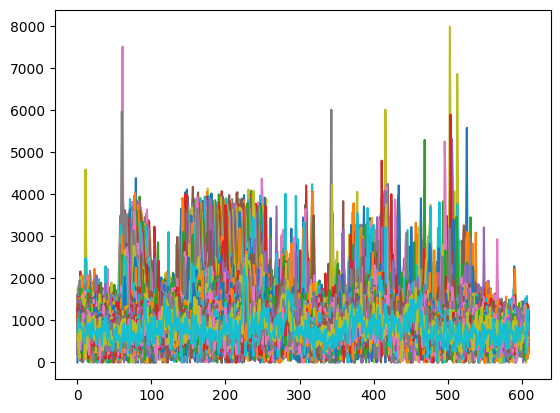
\includegraphics[scale=0.7]{fig9.png}
	\end{center}


می‌توانیم بصورت رندم نیز برای دیگر بخش‌ها این تصاویر را ایجاد کنیم:
\begin{latin}
	\begin{python}
plt.plot(pavia[:,:,random.randrange(0, 103)])
plt.show
	\end{python}
\end{latin}
\begin{center}
	\begin{figure}[H]
		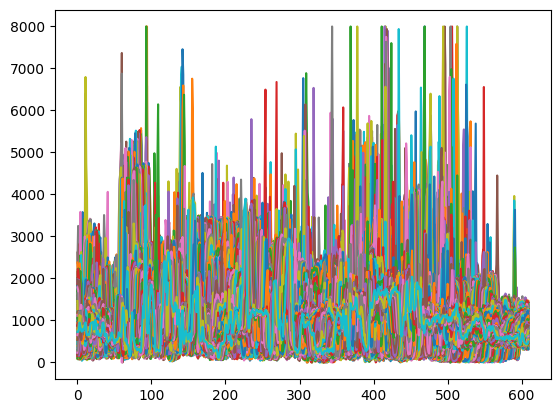
\includegraphics[scale=0.6]{fig10.png}
		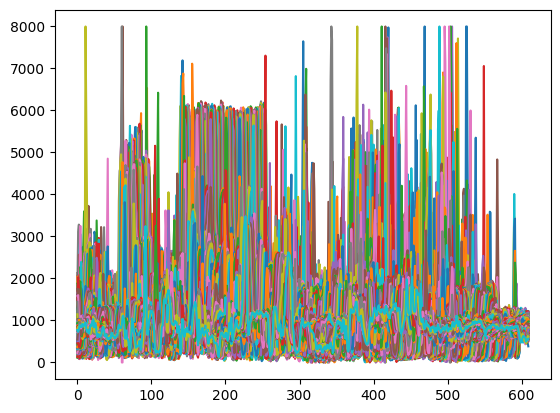
\includegraphics[scale=0.6]{fig11.png}
	\end{figure}
\end{center}
در نهایت می‌توانیم این داده‌ها را بصورت یک دیتافریم درآوریم .خوبی اینکار این است که می‌توانیم کار‌های طبقه‌بندی و خوشه‌بندی روی این دیتافریم‌ها انجام دهیم. برای اینکار لازم است که ابتدا آن را به ۲ بعدی تبدیل کنیم. 
\begin{latin}
	\begin{python}
pavia_rshp = pavia.reshape(207400,103)
pavia_df = pd.DataFrame(pavia_rshp)
pavia_df
	\end{python}
\end{latin}
\begin{latin}
	\begin{python}
paviagt_df = pd.DataFrame(paviagt)
paviagt_df
	\end{python}
\end{latin}
خروجی این کد ها را می‌توانید در فایل‌های کد ارائه شده در این گزارش مشاهده کنید و خودتان اجرا بگیرید.


\section*{تمرین سوم}

\subsection*{پیش‌گفتار}
اطلاعات جامعی از لینک اصلی این چالش یعنی
\href{http://clopinet.com/isabelle/Projects/NIPS2003/#challenge}{\lr{NIPS 2003}}
قابل دسترسی می‌باشد. در اینجا خلاصه‌ای از آن مطالب آورده خواهد شد. البته لازم به ذکر است اغلب مواردی را که سوال خواسته است در هماین سایت کامل آورده شده است و در اینجا من فقط آن‌ها را ترجمه کرده‌ام.

\subsection*{پس‌زمینه}
اخیرا (که مال سال ۲۰۰۳ است) تلاش‌های زیادی روی استخراج ویژگی 
\footnote{\lr{feature extraction}}
صورت گرفته است. در سال‌های گذشته، مقالات متعددی در این حوزه، شامل ساخت ویژگی‌ها
\footnote{\lr{feature construction}}
، کاهش ابعاد (فضایی)
\footnote{\lr{space dimensionality reduction}}
، نمایش تنکی
\footnote{\lr{sparse representation}}
و انتخاب ویژگی
\footnote{\lr{feature selection}}
 ، بیش از ۱۰ درصد ارسالی‌های NIPS را در بر می‌گرفتند و کاربر‌های زیادی در موضوعاتی چون بیوانفورماتیک 
 \footnote{\lr{bioinformatics}}
 ، شیمی، پردازش متن، تشخیص الگو ، تشخیص گفتار و دیدار داشتند.
 
 هدف از این کارگاه اشتراک تکنیک‌ها و متد‌ها است.  بخشی از این کارگاه به نمایش و بحث در خصوص نتجه چالش‌های انتخاب ویژگی می‌پردازد.نتایج بدست آمده در انتخاب ویژگی مربوط به دوران گذشته ، روی دیتاست‌های مختلف و شکاف‌های مختلف ، می‌باشند لذا مقایسه آن‌ها را سخت می‌کند.  برای اینکار یکسری دیتاست (در اینجا ۵ تا)  بصورت آزمون محک برای انتخاب ویژگی استفاده می‌شوند و لذا امکان کنترل آن‌ فراهم می‌گردد. این دیتاست‌ها هم به اندازه کافی بزرگ هستند تا نتایج بدست آمده امکان تایید از سمت امار را داشته باشد. ورودی‌ها متغیر‌هایی پیوسته یا دودوئی ، بصورت تنک یا چگال، هستند  همه مسائل بصورت مسئله طبقه‌بندی دوکلاسه است . 
 
 \subsection*{چالش اصلی}
 چالش اصلی در پیدا کردن الگوریتمی برای انتخاب ویژگی است که از متد‌هایی که از همه ویژگی‌ها استفاده میکنند، بهتر عمل کند. برای اینکار از ۵ دیتاست استفاده می‌شود و برای سادگی بیشتر نیز مسئله مورد بررسی یک طبقه‌بندی دوکلاسه‌ است. 
 
 \subsection*{نمره‌دهی}
 ارسالی‌هایی برای نمره‌دهی در نظر گرفته می‌شدند که پیش‌بینی کلاس (برچسب) برای 
 مجموعه‌های آموزش 
 \footnote{\lr{training}}
 و ارزیابی
 \footnote{\lr{validation}}
 یا 
 Val
 و آزمون
 \footnote{\lr{test}}
  ، برای هر ۵ دیتاست، و لیستی از ویژگی‌های استفاده شده 
 ارائه داده باشند. ارائه مقدار اطمینان طبقه‌بندی دلبخواهی بوده است. عملکرد آن‌ها توسط این معیار‌ها سنجیده می‌شود :
 \begin{itemize}
 	\item
 	BER :
 	نرخ بالانس خطا
 	\footnote{\lr{balance error rate}}
 	.
 	که در حقیقت میانگین نرخ خطای کلاس‌های مثبت و نرخ خطای کلاس‌های منفی است. چون برخی دیتاست‌ها از جمله 
 	Dorothea
 	ناهمگن هستند، از این معیار استفاده شده است.
 	\item
 	AUC
 	:
 	مساحت زیر منحنی ROC. منحنی ROC با تغییر یک آستانه در مقادیر متمایز (خروجی‌های) طبقه‌بند بدست می‌آیند. این منحنی نمایان‌گر کسر مثبت درست به کسر منفی غلط است . در طبقه‌بند های دودوئی، 
 	$BER = 1 - AUC$
 	می‌باشد.
 	\item
 	Ffeat
 	:
 	کسر ویژگی‌های انتخاب شده
 	\item
 	Fprob
 	:
 	کسر prob ‌های پیدا شده در مجموعه ویژگی‌های انتخاب شده. 	
 \end{itemize}

از این معیار‌ها برای نمره‌دهی استفاده می‌شود. برای رتبه‌بندی شرکت‌کنندگان، از نتایج مجموعه آزمون  ، به وسیله نمره‌ای که از تلفیق 
BER
،
Ffeat
و
Fprob
بدست می‌آید، استفاده می‌کنند. 
\begin{itemize}
	\item 
	دو به دو طبقه‌بند ها را برای هر دیتاست مقایسه می‌کنند.
	\item
	از آزمون 
	McNemar
	با نرخ ریسک ۵ درصد، برای مقایسه  بهتر بودن یک طبقه‌بند نسبت به طبقه‌بند دیگر، استفاده می‌کنند. نمره بدست آمده بصورت ۱ (اگر بهتر بود)، ۰ (اگر نمی‌دانیم) و ۱- (اگر بدتر بود) است.
	\item
	اگر نمره ۰ بود (در بالا)، یعنی آزمون قبل آن‌ها را یکی تشخیص داد، از 
	Ffeat
	در صورتی که اختلاف آن‌ها از ۵ درصد بیشتر باشد، استفاده می‌کنیم
	.
	\item
	اگر نمره ۰ بود، از 
	Fprob
	استفاده می‌کنیم.
	\item
	نمره نهایی شامل جمع نمره‌های مقایسه‌های دوبه‌دو است که توسط بالا‌ترین نمره بدست آمده نرمال‌سازی می‌شود. (برای هر دیتاست)
	\item
	نمره نهایی جامع، میانگین نمره‌های نهایی دیتاست‌هاست. 
	
\end{itemize}
 با این روش نمره‌های مثبت و منفی و حتی ۰ بدست می‌آوریم. 
 یکی از مشکلات این شکل نمره‌دهی  این است که اگر یک طبقه‌بند جدید وارد چالش شود، همه نمره‌ها تغییر می‌کند. 
 
 \subsection*{نتایج}
 در این بخش رتبه‌های برتر در تاریخ ۱ دسامبر، نمایش داده می‌شود. همچنین نمره نهایی آن‌ها و مقدار هر معیار برای آن‌ها، نام فردی که روی آن کار کرده است و روش استفاده آن آورده خواهد شد. نمره‌ها در ۱۰۰ ضرب شده‌اند.
 BER
 شامل نرخ خطای همگن (به درصد) می‌باشد. 
 AUC
 مساحت زیر منحنی ROC می‌باشد که در ۱۰۰ ضرب شده است.
 Fe
 درصد ویژگی‌های استفاده شده است.
 Pr
 درصد prob های در ویژگی‌های انتخاب شده است.
 
 \begin{latin}
 	\begin{center}
 		\begin{tabular}{|c|c|c|c|c|c|c|}
 			\hline
 			method&
 			people&
 			score &
 			BER & AUC& Fe & Pr
 			\\\hline
 			BayesNN-DFT 
 			&
 			Neal/Zhang
 			&
 			88.0
 			&
 			6.84
 			&
 			97.22
 			&
 			80.3
 			&
 			47.8
 			\\\hline
 			BayesNN-DFT & Neal/Zhang & 86.2 & 6.87 & 97.21 & 80.3 & 47.8
 			\\\hline
 			BayesNN-small & Neal & 68.7 & 8.20 & 96.12 & 4.7 & 2.9
 			\\\hline
 			BayesNN-large& Neal& 59.6 &8.21 & 96.36 
 			& 60.3 & 28.5
 			\\\hline
 			RF+RLSC & Torkkola/Tuv& 59.3& 9.07&  90.93& 22.5& 17.5
 			\\\hline
 			final2 &Chen &52.0 &9.31 &90.69 & 24.9 &12.0
 			\\\hline
 			SVMBased3 &Zhili/Li& 41.8 &9.21&93.60 &29.5& 21.7
 			\\\hline
 			SVMBased4 & Zhili/Li&  41.1& 9.40 & 93.41 & 29.5 &21.7
 			\\\hline
 			final1 &Chen& 40.4 &10.38& 89.62&  6.2& 6.1
 			\\\hline
 			transSVM2 &Zhili& 36.0& 9.60&  93.21&  29.5& 21.7
 			\\\hline
 			BayesNN-E &Neal& 29.5& 8.43& 96.30 & 96.8& 56.7
 			\\\hline
 			Collection2 & Saffari& 28.0& 10.03&  89.97 & 7.7 &10.6
 			\\\hline
 			Collection1 &Saffari &20.7 &10.06& 89.94&32.3 & 25.5
 			\\\hline
 		\end{tabular}
 		
 	\end{center}
 \end{latin}
بطور مشابه هم برای تاریخ ۸ دسامبر این رتبه‌بندی انجام شده‌ است و در مقاله اصلی قابل مشاهده است.

همچنین می‌توان تیم‌های شرکت کننده را بطور کلی (روش‌های استفاده شده توسط آن‌ها) به جدول زیر تقسیم کرد. لازم به ذکر است که حروفی که در جدول زیر آورده می‌شود، ترجمه شوند.
\begin{itemize}
	\item 
	classifier 
	:
	نوع طبقه‌بند (۴ گروه)
	\begin{itemize}
		\item 
		N :
		شبکه‌های عصبی
		\item
		\lr{K} :
		مثل SVM یا سایر روش‌های کرنل
		\item
		T
		:
		درخت
		\item
		O 
		:
		دیگر
	\end{itemize}
	\item
	Fengine :
	موتوز انتخاب ویژگی‌ها (۳ گروه)
	\begin{itemize}
		\item 
		C :
		معیار تک متغییری شامل ضرایب همبستگی
		\item
		T :
		درخت ، مثل RF به عنوان فیلتر
		\item
		E :
		روش‌های تعبیه شده 
		\footnote{\lr{embedded}}
	\end{itemize}
	\item
	Fsearch :
	روش‌های جستجو  (۴ گروه)
	\begin{itemize}
		\item 
		E :
		تعبیه شده
		\item
		R
		:
		رتبه ویژگی
		\item
		B :
		حذف عقب‌رو
		\footnote{\lr{backward elimination}}
		\item
		S
		:
		جستجو مفصل
	\end{itemize}
\end{itemize} 

\begin{center}
	\begin{latin}
		\begin{tabular}{|c|c|c|c|c|c|}
			\hline
			Team & Classifier &  Fengine & Fsearch & Ensemble & Transduction 
			\\\hline
			Neal/Zhang & N/O& C/E& E &Yes& Yes
			\\\hline
			Torkkola/Tuv &K &T &R& Yes& No
			\\\hline
			Chen/Lin &K& C/T/E& R/E& No& No
			\\\hline
			Zhili/Li &K &C/E& E &No& Yes
			\\\hline
			Saffari &N &C &R &Yes& No
			\\\hline
			Ghostminer &K &C/T& B &Yes& No
			\\\hline
			Lal et al &K &C &R& No& No
			\\\hline
			CBAGroup &K &C &R &No& No
			\\\hline
			Bachrach/Navot &K/O &E &S &No &No
			\\\hline
		\end{tabular}
	\end{latin}
\end{center}
\subsection*{برنده}
در هر دو تاریخ، نفرات اول
رادولف نیل 
\footnote{\lr{ Radford Neal}}
و
جیانگو ژنگ
\footnote{\lr{Jianguo Zhang }} 
 بودند. روش آن‌ها شامل تلفیق شبکه‌های عصبی بیزی
 \footnote{\lr{Bayesian neural networks}}
 و درخت پخش دریخت
 \footnote{\lr{Dirichlet diffusion trees}}
 بودند. نه تنها روش آن‌ها نمره خوبی به نسبت سایر شرکت کنندگان داشت بلکه مجموعه ویژگی‌هایی که استفاده کرده بودن نیز کوچکترین بود. توضیحات بیشتر در مورد روش آن‌ها در مقاله این چالش آورده شده است.
 
 
\subsection*{دیتاست}
مشخاصت دیتاست شامل نام ، دامنه استفاده، نوع داده (تنگ و چگال)، تعداد ویژگی‌ها، درصد prob ‌ها 
%\footnote{\lr{probes}}
، تعداد داده‌های آموزش ، داده‌های ارزیابی و داده‌های تست آورده شده است.
\begin{latin}
	\begin{center}
		\begin{tabular}{|c|c|c|c|c|c|c|c|}
			\hline
			Dataset & Domain & Type & Fe  & Pro  & Tr  & Val  & Te \\\hline
			
			Arcene& Mass Spectrometry &Dense &10000 &30 &100& 100 &700
			\\\hline
			Dexter &Text classification& Sparse &20000& 50& 300 &300& 2000
			\\\hline
			Dorothea& Drug discovery &Sparse binary &100000 &50 &800& 350& 800
			\\\hline
			Gisette& Digit recognition &Dense& 5000& 30 &6000& 1000& 6500
			\\\hline
			Madelon &Artificial &Dense& 500 &96 &2000 &600 &1800
			\\\hline
		\end{tabular}
	\end{center}
\end{latin} 

همه دیتاست‌ها در ابتدا به سه زیر مجموعه آموزش، ارزیابی و آزمون شکسته می‌شوند. از مجموعه تست برای نمره‌دهی نهایی استفاده می‌شود و مجموعه ارزیابی برای ، ارزیابی  عملکرد استفاده می‌شود.

همانطور که گفتیم تا اواخر دهه ۱۹۹۰، مقاله‌هایی که در مورد انتخاب ویژگی بودند، دیتاست‌هایی با کمتر از ۴۰ ویژگی را مورد بررسی قرار می‌دادند اما سال‌های بعد این شرایط تغییر کرد. این ۵ دیتاست نیز برای آزمون الگوریتم‌های انتخاب، مرتب شده‌اند. 

دیتاست‌ها از دامنه‌ها و سختی‌های متفاوتی  می‌آیند. متغییر‌های ورودی‌ آن‌ها در برخی پیوسته یا گسسته  ، تنگ یا چگال است ؛ یکی از دیتاست‌ها ناهمگن است. یکی دیگر 
،
MADELON
، 
بصورت مصنوعی برای نشان دادن یک مشکل خاص، طراحی شده است (انتخاب مجموعه‌ای از ویژگی‌ها بطوری که هیچ ویژگی به تنهایی اطلاعاتی ندارد). همانطور که قبلا نیز اشاره شد، دیتاست‌ها مثال‌های زیادی دارند تا آزمون آن از نظر آماری به مشکل نخورد. 

برای اینکه افرادی که قبلا این دیتاست‌ها را دیده‌اند، برتری بر دیگران نداشته باشند،  هویت این دیتاست ها در این آزمون محک، پنهان شده است. 

چندین پیش پردازش 
%\footnote{\lr{preprocessing}}
و فرمت کردن داده روی داده‌ها برای متمایز شدن مبدا آن‌ها انجام داده شده است. 


بطور خاص، ما تعدادی از ویژگی‌ها را به عنوان probe معرفی می‌کنیم. در ابتدا آن‌ها بصورت تصادفی انتخاب شده‌اند (بصورت تصادفی از توزیعی که به توزیع ویژگی‌ها شبیه باشد)، اما هیچ اطالاعاتی در مورد برچسب ها (کلاسها) با خود همراه ندارند. این prob ‌ها در ارزیابی عملکرد استفاده می‌شوند.  



\subsection*{پیش پردازش}
مرکزی کردن و مقیاس کردن ویژگی‌ها از جمله پیش پردازش‌هایی بود که بیشترین استفاده را داشت. برخی روش‌ها نیاز به گسسته‌سازی ویژگی ها داشتند. یک گروه از الگوها را نرمال کرد. آنالیز مولفه‌های اصلی 
\footnote{\lr{Principal Componant Analysis}}
یا PCA توسط چندین گروه انجام شد (همچین برنده هم از این روش برای ساخت ویژگی‌ها استفاده کرده بود). 

سه روش نرمال سازی شامل : 
\begin{itemize}
	\item 
	normalize1 :
	هر ویژگی جداگانه استاندارد شده (منهای میانگین تقسیم بر std به علاوه عامل fudge ) . زمانی که داده تنک یا sparse است، دیگر میانگین کسر نمی‌شود.
	\item
	normalize2 :
	 هر مثال به نرم ۲ آن تقسیم می‌شود
	\item
	normalize3 :
	هر مثال  به میان‌ نرم ۲‌های همه مثال‌ها تقسیم می‌شود.
\end{itemize}
بررسی کردن که 
normalize2
به نسبت بقیه بهتر عمل می‌کند.

\subsection*{نتیجه‌گیری}
این چالش نشان داد که انتخاب ویژگی می‌توان به خوبی (بطور موثر) انجام شود و حذف ویژگی‌های بی معنی برای بدست آوردن عملکر خوب در طبقه‌بندی واجب نیست.  در طراحی دیتاست‌ها تعداد زیادی ویژگی‌های پرت ، که آن‌ها را prob نامیدیم، آورده شده‌اند. در مقابل با ویژگی‌های اضافی که ممکن هم هست دقت را بهبود ندهند اما اطلاعات حمل می‌کنند، آن‌ها نویز سفید
\footnote{\lr{pure noise}}
هستند.  این چالش توانست قدرت روش‌های فیلترینگ را نمایش دهد. از طرفی می‌گویند روش‌های تعبیه شده بسیار توانا هستند ولی از نظر محاسباتی پر هزینه هستند. نتیجه مهم دیگری که بدست آمد این بود که طبقه‌بند های غیر خطی لزوما بیش‌برازی ندارند. 

\section*{لینک‌های مفید}

منبع بیشتر از google scholar و wikipedia  دریفات شده اند. 
علاوه بر این موارد می‌توانید اگر بنابر هر دلیلی فایل‌های ارائه شده، قابل به استفاده نبود، آن‌ها را از لینک زیر دانلود کنید. در نظر داشته باشید که در بین داده‌ها چون داده‌های pavia حجیم هستند، این داده را باید دستی دانلود کنید. 
این موارد برای زمانی است که فایل‌های اصلی که در سایت تمرین آپلود شده‌اند ، اجرا نشوند یا با مشکل دانلود شوند.

لینک :
\href{https://drive.google.com/drive/folders/1Cbyk2rJ3-KZH08Wu43DTUZTl_uWAqt2_?usp=sharing}{\lr{google drive}}


\end{document}


